\label{sec:appendix}
\subsection{Model Generation Approach}
oBERTa models are generated in a multi-stage approach with details found in figure \ref{fig:framework}
\begin{figure*}[!t]
    \centering
    \scalebox{0.7}{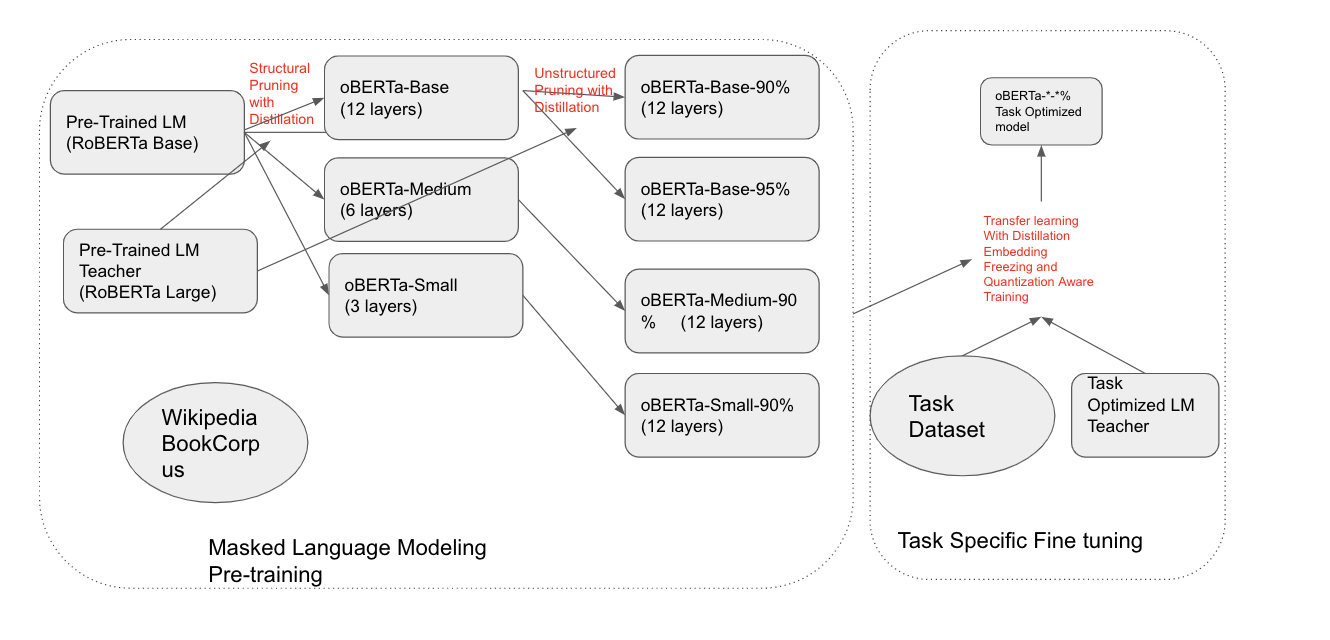
\includegraphics{oberta1.png}}
    \caption{The set of oBERTa language models follows a compounding compression approach. First models are structurally pruned and further pre-trained using KD and a RoBERTa\textsubscript{large}  teacher. Next, each model is pruned during additional pre-training to a target sparsity. After  pruning, the sparsity pattern is locked, and models are fine-tuned with KD on specialized NLP tasks. During fine-tuning, models may be quantized for additional improvements in inference efficiency.}
    \label{fig:framework}
\end{figure*}
\subsection{Roberta and Training Methodology}
RoBERTa \cite{Liu2019RoBERTaAR} is a language model that can best be considered more robust and optimized for the popular BERT model. While the models share architectures, their training differs as RoBERTA uses a 160 GB corpus for 10 epochs compared to the 4GB one used by BERT. As a result, the training time of RoBERTA is about 100 times higher than its predecessor.\\
Given this high cost of training and the regular need for longer training when pruning a model \cite{Kurti2022TheOB}, we focus on compressing RoBERTa without following its expensive pre-training regime. Our research leverages the popular open-source compression library SparseML\footnote{https://github.com/neuralmagic/sparseml} to implement unstructured pruning, structured pruning, and quantization via quantization-aware training. In all our experiments, we prune each network component independently using either GMP or Optimal BERT Surgeon (OBS) (Kurtic et al.). One exception is the embeddings layer, which we do not prune.\\
\subsection{Model Details}
Model details can be found in table \ref{tab:oberta-model-info}
\begin{table*}[!tb]
    \centering
    \scalebox{0.65}{
    \begin{tabular}{|l|l|l|l|l|l|l|l|l|}
    \hline
        Model & Parameters & Prunable & Sparse & Sparsity & size (MB) & Compression & GZIP size (MB) & Compression \\ \hline
        oBERTa\textsubscript{base} & 124,647,170 & 85,526,016 & 1,539 & 0.0\% & 474 & 1.00 & 435 & 1.00 \\ \hline
        oBERTa\textsubscript{base} Quantized & 124,647,170 & 85,526,016 & 1,539 & 0.0\% & 119 & 3.98 & 85 & 5.12 \\ \hline
        oBERTa\textsubscript{base} 90\% & 124,647,170 & 85,526,016 & 76,442,738 & 89.4\% & 474 & 1.00 & 183 & 2.38 \\ \hline
        oBERTa\textsubscript{base} 90\% Quantized & 124,647,170 & 85,526,016 & 76,442,738 & 89.4\% & 119 & 3.98 & 42 & 10.36 \\ \hline
        oBERTa\textsubscript{base} 95\% & 124,647,170 & 85,526,016 & 80,689,466 & 94.3\% & 474 & 1.00 & 163 & 2.67 \\ \hline
        oBERTa\textsubscript{base} 95\% Quantized & 124,647,170 & 85,526,016 & 80,689,466 & 94.3\% & 119 & 3.98 & 37 & 11.76 \\ \hline
        oBERTa\textsubscript{MEDIUM} & 82,119,938 & 43,058,688 & 1,538 & 0.0\% & 312 & 1.52 & 289 & 1.51 \\ \hline
        oBERTa\textsubscript{MEDIUM} Quantized & 82,119,938 & 43,058,688 & 1,538 & 0.0\% & 78 & 6.08 & 53 & 8.21 \\ \hline
        oBERTa\textsubscript{MEDIUM} 90\%   & 82,119,938 & 43,058,688 & 38,222,138 & 88.8\% & 312 & 1.52 & 161 & 2.70 \\ \hline
        oBERTa\textsubscript{MEDIUM} 90\% Quantized  & 82,119,938 & 43,058,688 & 38,222,138 & 88.8\% & 78 & 6.08 & 33 & 13.18 \\ \hline
        oBERTa\textsubscript{SMALL} & 60,856,322 & 21,825,024 & 1,538 & 0.0\% & 233 & 2.03 & 214 & 2.03 \\ \hline
        oBERTa\textsubscript{SMALL} Quantized & 60,856,322 & 21,825,024 & 1,538 & 0.0\% & 60 & 7.90 & 39 & 11.15 \\ \hline
        oBERTa\textsubscript{SMALL} 90\% & 60,856,322 & 21,825,024 & 19,111,068 & 87.6\% & 233 & 2.03 & 149 & 2.92 \\ \hline
        oBERTa\textsubscript{SMALL} 90\% Quantized & 60,856,322 & 21,825,024 & 19,111,838 & 87.6\% & 60 & 7.90 & 30 & 14.50 \\ \hline
    \end{tabular}}
    \caption{Description of the oBERTa model family and their sparsity and size. Prunable parameters are the sum of all non-embedding parameters in the model. Since sparsity profiles are assigned at a module level, overall sparsity profiles do not perfectly match the target 90\% or 95\% which are targeted.}
    \label{tab:oberta-model-info}
\end{table*}
\subsection{Dataset Details}
\label{sec:datasets}
Dataset statistics are detailed in Table \ref{tab:dataset_stat}.
\begin{table}[!htb]
      \centering
         {\small 
             \begin{tabular}{l|c|c}
                \toprule 
                Dataset & Train & Eval \\
                \midrule
                SQuAD v1.1 (examples) &  87599 & 10570\\
                SQuAD v2.0 (examples) &  130319	 & 11873\\
                \midrule
                MNLI (examples) & 392702 & 19628 \\
                \midrule
                QQP (examples) &  363,846 & 40,430 \\
                \midrule
                IMDB (examples) & 25000	 & 25000 \\
                \midrule
                CONLL2003 (examples) & 14041	 & 3250 \\
                \midrule
                SST2 (examples) & 67349	 & 872	 \\
                \midrule
                Wikipedia (words) & 6078422  & - \\
                \midrule
                TBC (words) & 74004228 & - \\ 
                \bottomrule
            \end{tabular}
         }
     \caption{Statistics for training and evaluation datasets}
    \label{tab:dataset_stat}
\end{table}
\subsection{Teacher models}
\label{sec:TeacherStats}
Performance of the RoBERTa\textsubscript{base}and RoBERTa\textsubscript{large} models on our sparse transfer datasets. We explore the optimal hyperparameters relative to performance in published results as shown in table \ref{tab:teacher-base} and \ref{tab:teacher-large}
\begin{table*}[!ht]
    \centering
    \scalebox{0.7}{
    \begin{tabular}{|l|l|l|l|l|l|l|l|l|l|l|}
    \hline
        Model & Training Epochs & Batch Size & Learning Rate & Weight Decay & Warmup & Target Metric & Target Score & Actual & Recall \\ \hline
        SQUAD V1.1 & 3 & 16 & 1.00E-05 & 0 & 0  & F1 & 90.40 & 92.15 & 101.94\% \\ \hline
        SQUAD V2.0  & 3 & 16 & 3.00E-05 & 0 & 0 & F1 & 82.91 & 83.53 & 100.74\% \\ \hline
        QQP & 5 & 16 & 2.00E-05 & 0 & 0 & ACC & 91.90 & 91.52 & 99.59\% \\ \hline
        MNLI & 3 & 16 & 1.00E-05 & 0 & 0 &  ACC & 87.60 & 87.88 & 100.31\% \\ \hline
        SST-2 & 3 & 16 & 2.00E-05 & 0 & 0 &  ACC & 94.80 & 94.61 & 99.80\% \\ \hline
        CONLL2003 & 3 & 16 & 3.00E-05 & 0 & 0 &  ACC & 99.10 & 99.29 & 100.19\% \\ \hline
        IMDB & 3 & 16 & 1.00E-05 & 0 & 0 &  ACC & 94.67 & 95.24 & 100.60\% \\ \hline
    \end{tabular}}
    \caption{Training parameters along with performance metrics and the recovery vs. the published performance of the same model for the RoBERTa base model}
    \label{tab:teacher-base}
\end{table*}
\begin{table*}[!ht]
    \centering
    \scalebox{0.7}{
    \begin{tabular}{|l|l|l|l|l|l|l|l|l|l|l|}
    \hline
        Model & Training Epochs & Batch Size & Learning Rate & Weight Decay & Warmup &Target Metric & Target Score & Actual & Recall \\ \hline
        SQUAD V1.1 & 3 & 16 & 1.00E-05 & 0 & 0  & F1 & 94.50 & 94.62 & 100.12\% \\ \hline
        SQUAD V2.0  & 3 & 16 & 1.00E-05 & 0 & 0  & F1 & 89.40 & 89.14 & 99.71\% \\ \hline
        QQP & 3 & 16 & 1.00E-05 & 0 & 0 &  ACC & 92.20 & 91.76 & 99.52\% \\ \hline
        MNLI & 3 & 16 & 1.00E-05 & 0 & 0 &  ACC & 90.20 & 90.61 & 100.45\% \\ \hline
        SST-2 & 3 & 16 & 1.00E-05 & 0 & 0 &  ACC & 96.40 & 96.22 & 99.81\% \\ \hline
        CONLL2003 & 3 & 16 & 3.00E-05 & 0 & 0 &  ACC & 99.10 & 99.39 & 100.29\% \\ \hline
        IMDB & 3 & 16 & 1.00E-05 & 0 & 0 &  ACC & 94.67 & 96.12 & 101.53\% \\ \hline
    \end{tabular}}
    \caption{Training parameters along with performance metrics and the recovery vs. the published performance of the same model for the RoBERTa large model}
    \label{tab:teacher-large}
\end{table*}
\subsection{Upstream Pruning}
Following the findings that more extensive teachers distill better \cite{Liu2019RoBERTaAR} and our experiments, we use both RoBERTa\textsubscript{base}and RoBERTa\textsubscript{large} as teachers eventually find the large model works better. Using this teacher, we use the parameters shown in table \ref{tab:hyperparams-UpstreamPruning} to prune the models for oBERTa. This same set of parameters is applied to the structurally pruned models, but there is no induced sparsity. 
\begin{table*}
      \centering
         {\small 
            \begin{tabular}{l|c}
            \toprule
            & 5 Epochs \\
            \midrule
            Datasets & BookCorpus \& English Wikipedia \\
            \midrule
            Batch size & 256 \\
            \midrule
            Initial learning rate & 5e-4 \\
            Learning rate schedule & linear decay with rewinds \\
            Learning rate rewinds & periodic every 0.5 epochs \\
            \midrule
            Max sequence length & 512 \\
            Weight decay & 0.01 \\
            \midrule
            \makecell{Knowledge Distillation\\(hardness, temperature)} & (1.0, 5.5) \\
            \midrule
            Student model & dense oBERTa-* model \\
            Teacher model & RoBERTa\textsubscript{large} \\
            \midrule
            Pruning frequency & 100x per epoch \\
            \bottomrule
            \midrule
            Initial Sparsity & 0.7 for 12 layer model, 0.5 for the 6-layer, and 0.3 for the 3-layer \\
            \bottomrule
            \end{tabular}
        }
            \caption{Upstream pruning hyper-parameters.}
            \label{tab:hyperparams-UpstreamPruning}
\end{table*}
\subsection{Sparse Transfer Hyper-parameters}
\label{sec:downstream}
Our work aims not to produce the highest possible performance of a sparse language model. Instead, we aim to make light language models that perform well on various tasks with minimal hyperparameter optimization. As a result, in all of our experiments, we leverage the parameters shown in \ref{tab:hyperparams-transfer} and \ref{tab:hyperparams-transfer-quant} and perform a grid search over them. 
\begin{table*}
      \centering
        {\small 
            \begin{tabular}{l|c}
            \toprule
            & 10 Epochs \\
            \midrule
            Initial learning rate & \makecell{2.1e-4,1.9e-4,1.7e-4,1.5e-4,1.3e-4,1.1e-4,9e-5,7e-5,5e-5,3e-5,2e-5,1e-5} \\
            Learning rate schedule & linear decay to 0 \\
            \midrule
                Batch size & 12 \\
            \midrule
            \midrule
                Weight Decay & \makecell{0.0, 0.01, 0.05, 0.1} \\
            \midrule
            \midrule
               Knowledge Distillation hardness & \makecell{1.0, 0.0} \\
            \midrule
            \midrule
               Frozen Embeddings & \makecell{1.0, 0.0} \\
            \midrule
            \midrule
               Knowledge Distillation temperature & 7.0 \\
            \midrule
            \midrule
               Knowledge Distillation Teacher & \makecell{RoBERTa\textsubscript{base}, RoBERTa\textsubscript{large}} \\
            \midrule
            \bottomrule
            \end{tabular}
        }
        \caption{Sparse-transfer learning hyper-parameters used to fine-tune upstream-pruned models at downstream tasks. Each Experiment tunes this set of parameters to find a task-specific optimal combination.}
    \label{tab:hyperparams-transfer}
\end{table*}
\begin{table*}
      \centering
        {\small 
            \begin{tabular}{l|c}
            \toprule
            & 20 Epochs \\
            \midrule
            Initial learning rate & \makecell{2.1e-4,1.9e-4,1.7e-4,1.5e-4,1.3e-4,1.1e-4,9e-5,7e-5,5e-5,3e-5,2e-5,1e-5} \\
            Learning rate schedule & linear decay to 0. Rewind to 5e-5 for QAT at epoch 10 \\
            \midrule
                Freeze Batch Norm Epoch & 18 \\
            \midrule
            \midrule
                Batch size & 12 \\
            \midrule
            \midrule
                Weight Decay & \makecell{0.0, 0.01, 0.05, 0.1} \\
            \midrule
            \midrule
               Knowledge Distillation hardness & \makecell{1.0, 0.0} \\
            \midrule
            \midrule
               Frozen Embeddings & \makecell{1.0, 0.0} \\
            \midrule
            \midrule
               Frozen Embeddings Schedule & Frozen until epoch 10, unfrozen for QAT \\
            \midrule
            \midrule
               Knowledge Distillation temperature & 7.0 \\
            \midrule
            \midrule
               Knowledge Distillation Teacher & \makecell{RoBERTa\textsubscript{base}, RoBERTa\textsubscript{large}} \\
            \midrule
            \bottomrule
            \end{tabular}
        }
        \caption{Sparse-transfer learning with Quantization hyper-parameters used to fine-tune upstream-pruned models at downstream tasks. Each Experiment tunes this set of parameters to find a task-specific optimal combination.}
    \label{tab:hyperparams-transfer-quant}
\end{table*}
\subsection{Learning Rate}
\label{sec:sparse-transfer-learning-rate}
In our exploration of sparse transfer learning, we perform a wide study on the impact of the optimal learning rate for each task and each model in the oBERTa family. The results as shown in table \ref{tab:learning-rate}
\begin{table*}
      \centering
        {\small 
        \begin{tabular}{|l|l|l|l|l|l|l|l|}
    \hline
         & \multicolumn{7}{l}{Optimal Learning Rate} \\ \hline
        model & SQUAD & SQUAD V2 & MNLI & QQP & IMDB & SST2 & CONLL2003 \\ \hline
        RoBERTa\textsubscript{base}& 1.00E-05 & 3.00E-05 & 1.00E-05 & 2.00E-05 & 1.00E-05 & 2.00E-05 & 3.00E-05 \\ \hline
        RoBERTa\textsubscript{large} & 1.00E-05 & 1.00E-05 & 1.00E-05 & 1.00E-05 & 1.00E-05 & 1.00E-05 & 3.00E-05 \\ \hline
        oBERTa\textsubscript{base}& 1.00E-05 & 1.00E-05 & 1.00E-05 & 2.00E-05 & 1.00E-05 & 2.00E-05 & 3.00E-05 \\ \hline
        oBERTa\textsubscript{base} 90\% & 1.50E-04 & 1.50E-04 & 7.00E-05 & 1.70E-04 & 1.30E-04 & 9.00E-05 & 1.50E-04 \\ \hline
        oBERTa\textsubscript{base} 95\% & 1.50E-04 & 1.30E-04 & 9.00E-05 & 2.10E-04 & 1.30E-04 & 9.00E-05 & 5.00E-05 \\ \hline
        oBERTa\textsubscript{MEDIUM} & 5.00E-05 & 5.00E-05 & 2.00E-05 & 3.00E-05 & 3.00E-05 & 2.00E-05 & 3.00E-05 \\ \hline
        oBERTa\textsubscript{MEDIUM} 90\%   & 1.50E-04 & 1.30E-04 & 1.50E-04 & 1.50E-04 & 5.00E-05 & 1.50E-04 & 1.50E-04 \\ \hline
        oBERTa\textsubscript{SMALL} & 1.50E-04 & 1.50E-04 & 3.00E-05 & 5.00E-05 & 3.00E-05 & 5.00E-05 & 3.00E-05 \\ \hline
        oBERTa\textsubscript{SMALL} 90\% & 1.50E-04 & 1.50E-04 & 2.10E-04 & 2.10E-04 & 1.50E-04 & 2.10E-04 & 1.90E-04 \\ \hline
    \end{tabular}    
        }
        \caption{Sparse-transfer learning with Quantization hyper-parameters used to fine-tune upstream-pruned models at downstream tasks. Each Experiment tunes this set of parameters to find a task-specific optimal combination.}
    \label{tab:learning-rate}
\end{table*}
\subsection{Knowledge Distillation}
\label{sec:sparse-transfer-KD}
In our exploration of sparse transfer learning, we perform a wide study on the impact of knowledge distillation. Across tasks, we look at the impact using no teacher, RoBERTa\textsubscript{base}and RoBERTa\textsubscript{large} as shown in tables \ref{tab:kd-mnli},\ref{tab:kd-qqp},\ref{tab:kd-sst},\ref{tab:kd-conll},\ref{tab:kd-squad},\ref{tab:kd-squad2}

\begin{table}[!htb]
    \centering
    \scalebox{0.7}{
    \begin{tabular}{|l|l|l|l|}
    \hline
        model & No KD & KD-Base & KD-Large \\ \hline
        oBERTa\textsubscript{base}(Target) & 91.52\% & N/A & N/A \\ \hline
        oBERTa\textsubscript{base} 90\% & 91.97 & 92.78 & 92.55 \\ \hline
        oBERTa\textsubscript{base} 95\% & 91.40 & 91.17 & 91.514 \\ \hline
        oBERTa\textsubscript{MEDIUM} & 90.94 & 91.86 & 91.78 \\ \hline
        oBERTa\textsubscript{MEDIUM} 90\% & 87.16 & 87.16 & 89.56 \\ \hline
        oBERTa\textsubscript{SMALL} & 89.56 & 88.65 & 90.83 \\ \hline
        oBERTa\textsubscript{SMALL} 90\% & 85.58 & 89.22 & 89.45 \\ \hline
    \end{tabular}}
    \caption{Impact of knowledge distillation on the accuracy (matched) MNLI Dataset across model sizes for the various sizes of oBERTa as compared to the regularly trained baseline}
    \label{tab:kd-mnli}
\end{table}

\begin{table}[!htb]
    \centering
    \scalebox{0.7}{
    \begin{tabular}{|l|l|l|l|}
    \hline
        model & No KD & KD-Base & KD-Large \\ \hline
        oBERTa\textsubscript{base}(Target) & 91.52 & N/A & N/A \\ \hline
        oBERTa\textsubscript{base} 90\% & 63.18 & 91.01 & 90.93 \\ \hline
        oBERTa\textsubscript{base} 95\% & 90.46 & 90.45 & 90.72 \\ \hline
        oBERTa\textsubscript{MEDIUM} & 90.75 & 90.96 & 90.96 \\ \hline
        oBERTa\textsubscript{MEDIUM} 90\% & 89.93 & 90.41 & 89.82 \\ \hline
        oBERTa\textsubscript{SMALL} & 86.63 & 87.34 & 87.65 \\ \hline
        oBERTa\textsubscript{SMALL} 90\% & 88.72 & 89.40 & 87.50 \\ \hline
    \end{tabular}}
    \caption{Impact of knowledge distillation on the accuracy QQP Dataset across model sizes for the various sizes of oBERTa as compared to the regularly trained baseline}
    \label{tab:kd-qqp}
\end{table}

\begin{table}[!htb]
    \centering
    \scalebox{0.7}{
    \begin{tabular}{|l|l|l|l|}
    \hline
        model & No KD & KD-Base & KD-Large \\ \hline
        oBERTa\textsubscript{base}(Target) & 91.52 & N/A & N/A \\ \hline
        oBERTa\textsubscript{base} 90\% & 91.97 & 92.78 & 92.55 \\ \hline
        oBERTa\textsubscript{base} 95\% & 91.4 & 91.17 & 91.514 \\ \hline
        oBERTa\textsubscript{MEDIUM} & 90.94 & 91.86 & 91.78 \\ \hline
        oBERTa\textsubscript{MEDIUM} 90\% & 87.16 & 87.16 & 89.56 \\ \hline
        oBERTa\textsubscript{SMALL} & 89.56 & 88.65 & 90.83 \\ \hline
        oBERTa\textsubscript{SMALL} 90\% & 85.58 & 89.22 & 89.45 \\ \hline
    \end{tabular}}
    \caption{Impact of knowledge distillation on the accuracy SST-2 Dataset across model sizes for the various sizes of oBERTa as compared to the regularly trained baseline}
    \label{tab:kd-sst}
\end{table}

\begin{table}[!htb]
    \centering
    \scalebox{0.7}{
    \begin{tabular}{|l|l|l|l|}
    \hline
        model & No KD & KD-Base & KD-Large \\ \hline
        oBERTa\textsubscript{base}(Target) & 91.52\% & N/A & N/A \\ \hline
        oBERTa\textsubscript{base} 90\% & 99.17 & 99.08 & 99.11 \\ \hline
        oBERTa\textsubscript{base} 95\% & 98.89 & 98.47 & 97.51 \\ \hline
        oBERTa\textsubscript{MEDIUM} & 99.21 & 99.16 & 99.19 \\ \hline
        oBERTa\textsubscript{MEDIUM} 90\% & 99.01 & 98.8 & 98.79 \\ \hline
        oBERTa\textsubscript{SMALL} & 99.05 & 98.95 & 98.94 \\ \hline
        oBERTa\textsubscript{SMALL} 90\% & 98.88 & 98.55 & 98.55 \\ \hline
    \end{tabular}}
    \caption{Impact of knowledge distillation on the accuracy on the CONLL2003 Dataset across model sizes for the various sizes of oBERTa as compared to the regularly trained baseline}
    \label{tab:kd-conll}
\end{table}

\begin{table}[!htb]
    \centering
    \scalebox{0.7}{
    \begin{tabular}{|l|l|l|l|}
    \hline
        model & No KD & KD-Base & KD-Large \\ \hline
        oBERTa\textsubscript{base}(Target) & 91.52\% & N/A & N/A \\ \hline
        oBERTa\textsubscript{base} 90\% & 89.01 & 90.86 & 90.92 \\ \hline
        oBERTa\textsubscript{base} 95\% & 87.06 & 89.84 & 89.21 \\ \hline
        oBERTa\textsubscript{MEDIUM} & 84.36 & 88.20 & 85.74 \\ \hline
        oBERTa\textsubscript{MEDIUM} 90\% & 84.71 & 89.26 & 88.61 \\ \hline
        oBERTa\textsubscript{SMALL} & 82.00 & 80.77 & 77.08 \\ \hline
        oBERTa\textsubscript{SMALL} 90\% & 73.31 & 84.66 & 83.13 \\ \hline
    \end{tabular}}
    \caption{Impact of knowledge distillation on the F1 SQUAD v1.1 Dataset across model sizes for the various sizes of oBERTa as compared to the regularly trained baseline}
    \label{tab:kd-squad}
\end{table}

\begin{table}[!htb]
    \centering
    \scalebox{0.7}{
    \begin{tabular}{|l|l|l|l|}
    \hline
         model & No KD & KD-Base & KD-Large \\ \hline
        oBERTa\textsubscript{base}(Target) & 91.52\% & N/A & N/A \\ \hline
        oBERTa\textsubscript{base} 90\% & 75.57852204 & 80.25256971 & 81.32561567 \\ \hline
        oBERTa\textsubscript{base} 95\% & 72.61 & 77.67 & 77.98 \\ \hline
        oBERTa\textsubscript{MEDIUM} & 69.42634 & 70.97328 & 71.55996 \\ \hline
        oBERTa\textsubscript{MEDIUM} 90\% & 68.25281 & 76.02975 & 76.64135 \\ \hline
        oBERTa\textsubscript{SMALL} & 66.8281 & 62.9573 & 63.1224 \\ \hline
        oBERTa\textsubscript{SMALL} 90\% & 55.3959 & 70.0796 & 70.7913 \\ \hline
    \end{tabular}}
    \caption{Impact of knowledge distillation on the F1 SQUAD v2.0 Dataset across model sizes for the various sizes of oBERTa as compared to the regularly trained baseline}
    \label{tab:kd-squad2}
\end{table}
\subsection{Freezing Embeddings}
\label{sec:sparse-transfer-freeze-embd}
In our exploration of sparse transfer learning, we perform a wide study on the impact of freezing the embeddings during finetuning. Across tasks, we look at the impact of frozen and unfrozen embeddings as shown in tables \ref{tab:mnli-freeze},\ref{tab:qqp-freeze},\ref{tab:sst2-freeze},\ref{tab:CONLL-freeze},\ref{tab:squad-freeze}, and \ref{tab:squad2-freeze}. Besides question answering, we do not find a strong trend with the impact of frozen embeddings. In some tasks, sparse and dense models perform better with frozen embeddings while not for others. Focusing on question answering, by using frozen embeddings dense models see large losses in F1 score and the opposite can be seen for pruned models.   
\begin{table}[!htb]
    \centering
    \scalebox{0.99}{
    \begin{tabular}{|l|l|l|}
    \hline
        model & Frozen & Unfrozen \\ \hline
        oBERTa\textsubscript{base} (Target) & N/A & 87.88\% \\ \hline
        oBERTa\textsubscript{base} 90\% & 84.50 & 83.81 \\ \hline
        oBERTa\textsubscript{base} 95\% & 83.91 & 83.41 \\ \hline
        oBERTa\textsubscript{MEDIUM} & 84.37 & 83.32 \\ \hline
        oBERTa\textsubscript{MEDIUM} 90\% & 81.61 & 77.00 \\ \hline
        oBERTa\textsubscript{SMALL} & 80.24 & 80.36 \\ \hline
        oBERTa\textsubscript{SMALL} 90\% & 78.46 & 74.25 \\ \hline
    \end{tabular}}
    \caption{Impact of frozen vs trained embeddings on the accuracy (matched) MNLI Dataset across model sizes for the various sizes of oBERTa as compared to the uncompressed baseline}
    \label{tab:mnli-freeze}
\end{table}
\begin{table}[!htb]
    \centering
    \begin{tabular}{|l|l|l|}
    \hline
        model & Frozen & Unfrozen \\ \hline
        oBERTa\textsubscript{base} (Target) & N/A & 91.52\% \\ \hline
        oBERTa\textsubscript{base} 90\% & 90.93\% & 90.99\% \\ \hline
        oBERTa\textsubscript{base} 95\% & 90.72\% & 90.85\% \\ \hline
        oBERTa\textsubscript{MEDIUM} & 90.96\% & 91.35\% \\ \hline
        oBERTa\textsubscript{MEDIUM} 90\% & 89.82\% & 90.48\% \\ \hline
        oBERTa\textsubscript{SMALL} & 90.59\% & 90.72\% \\ \hline
        oBERTa\textsubscript{SMALL} 90\% & 89.40\% & 89.74\% \\ \hline
    \end{tabular}
    \caption{Impact of frozen vs trained embeddings on the accuracy on QQP across model sizes for the various sizes of oBERTa as compared to the uncompressed baseline}
    \label{tab:qqp-freeze}
\end{table}
\begin{table}[!ht]
    \centering
    \begin{tabular}{|l|l|l|}
    \hline
    model & Frozen & Unfrozen \\ \hline   
    oBERTa\textsubscript{base} (Target) & N/A & 91.52\% \\ \hline
        oBERTa\textsubscript{base} 90\% & 92.55 & 91.74\\ \hline
        oBERTa\textsubscript{base} 95\% & 91.514 & 91.4 \\ \hline
        oBERTa\textsubscript{MEDIUM} & 91.78 & 92.89 \\ \hline
        oBERTa\textsubscript{MEDIUM} 90\% & 89.56 & 88.76 \\ \hline
        oBERTa\textsubscript{SMALL} & 90.83 & 90.48 \\ \hline
        oBERTa\textsubscript{SMALL} 90\% & 89.45 & 89.34 \\ \hline    
    \end{tabular}
    \caption{Impact of frozen vs trained embeddings on the accuracy SST2 Dataset across model sizes for the various sizes of oBERTa as compared to the uncompressed baseline}
    \label{tab:sst2-freeze}
\end{table}
\begin{table}[!ht]
    \centering
    \begin{tabular}{|l|l|l|}
    \hline
     model & Frozen & Unfrozen \\ \hline
        oBERTa\textsubscript{base} (Target) & N/A & 91.52\% \\ \hline
        oBERTa\textsubscript{base} 90\% & 97.51 & 98.55 \\ \hline
        oBERTa\textsubscript{base} 95\% & 99.11 & 99.13 \\ \hline
        oBERTa\textsubscript{MEDIUM} & 99.19 & 99.18 \\ \hline
        oBERTa\textsubscript{MEDIUM} 90\% & 98.79 & 98.9 \\ \hline
        oBERTa\textsubscript{SMALL} & 98.94 & 98.94 \\ \hline
        oBERTa\textsubscript{SMALL} 90\% & 98.55 & 98.69 \\ \hline
    \end{tabular}
    \caption{Impact of frozen vs trained embeddings on the accuracy on CONLL2003 Dataset across model sizes for the various sizes of oBERTa as compared to the uncompressed baseline}
    \label{tab:CONLL-freeze}
\end{table}

\begin{table}[!ht]
    \centering
    \begin{tabular}{|l|l|l|}
    \hline
        model & Frozen & Unfrozen \\ \hline
        oBERTa\textsubscript{base} (Target) & N/A & 91.52\% \\ \hline
        oBERTa\textsubscript{base} 90\% & 90.92 & 83.99 \\ \hline
        oBERTa\textsubscript{base} 95\% & 89.21 & 87.08 \\ \hline
        oBERTa\textsubscript{MEDIUM} & 85.74 & 89.95 \\ \hline
        oBERTa\textsubscript{MEDIUM} 90\% & 88.61 & 86.63 \\ \hline
        oBERTa\textsubscript{SMALL} & 77.08 & 84.64 \\ \hline
        oBERTa\textsubscript{SMALL} 90\% & 83.13 & 77.43 \\ \hline
    \end{tabular}
    \caption{Impact of frozen vs trained embeddings on SQUAD v1.1 F1 across model sizes for the various sizes of oBERTa as compared to the uncompressed baseline}
    \label{tab:squad-freeze}
\end{table}

\begin{table}[!ht]
    \centering
    \begin{tabular}{|l|l|l|}
    \hline
        model & Frozen & Unfrozen \\ \hline
        oBERTa\textsubscript{base} (Target) & N/A & 91.52\% \\ \hline
        oBERTa\textsubscript{base} 90\% & 71.56 & 78.05 \\ \hline
        oBERTa\textsubscript{base} 95\% & 81.33 & 78.45 \\ \hline
        oBERTa\textsubscript{MEDIUM} & 77.98 & 76.86 \\ \hline
        oBERTa\textsubscript{MEDIUM} 90\% & 76.64 & 72.77 \\ \hline
        oBERTa\textsubscript{SMALL} & 71.32 & 63.12 \\ \hline
        oBERTa\textsubscript{SMALL} 90\% & 70.79 & 59.38 \\ \hline
    \end{tabular}
    \caption{Impact of frozen vs trained embeddings on the SQUAD v2.0 Dataset across model sizes for the various sizes of oBERTa as compared to the uncompressed baseline}
    \label{tab:squad2-freeze}
\end{table}
\subsection{Inference Benchmarks}
\label{sec:sparse-transfer-params}
We provide full results for our experiments in benchmarking the impact of compression on inference efficiency as shown in tables \ref{tab:inference-competitive-full},\ref{tab:inference-bs-64-core4},\ref{tab:inference-bs-16-core4},\ref{tab:inference-bs-1-core24},\ref{tab:inference-bs-64-core24},\ref{tab:inference-bs-16-core24},\ref{tab:inference-bs-1-core4-competitive},\ref{tab:inference-bs-1-core4-competitive}
\begin{table*}[!ht]
    \centering
    \scalebox{0.60}{
    \begin{tabular}{|l|l|l|l|l|l|}
    \hline
        model & Throughput (items/sec) & Speedup & Latency Mean (ms/batch) & Latency Median (ms/batch & Latency Std (ms/batch) \\ \hline
        oBERTa\textsubscript{base} & 16.69 & 1.00 & 59.90 & 59.82 & 1.02 \\ \hline
        oBERTa\textsubscript{base} Quantized & 51.68 & 3.10 & 19.34 & 19.28 & 0.58 \\ \hline
        oBERTa\textsubscript{base} 90\% & 54.87 & 3.29 & 18.21 & 18.15 & 0.31 \\ \hline
        oBERTa\textsubscript{base} 90\% Quantized & 68.70 & 4.12 & 14.55 & 14.50 & 0.20 \\ \hline
        oBERTa\textsubscript{base} 95\% & 145.57 & 8.72 & 6.86 & 6.86 & 0.11 \\ \hline
        oBERTa\textsubscript{base} 95\% Quantized & 78.90 & 4.73 & 12.66 & 12.68 & 0.31 \\ \hline
        oBERTa\textsubscript{MEDIUM} & 32.78 & 1.96 & 30.49 & 30.44 & 1.19 \\ \hline
        oBERTa\textsubscript{MEDIUM} Quantized & 103.47 & 6.20 & 9.65 & 9.60 & 0.57 \\ \hline
        oBERTa\textsubscript{MEDIUM} 90\%   & 106.01 & 6.35 & 9.42 & 9.34 & 0.28 \\ \hline
        oBERTa\textsubscript{MEDIUM} 90\% Quantized  & 149.25 & 8.94 & 6.69 & 6.65 & 0.42 \\ \hline
        oBERTa\textsubscript{SMALL} & 64.93 & 3.89 & 15.39 & 15.31 & 0.66 \\ \hline
        oBERTa\textsubscript{SMALL} Quantized & 208.09 & 12.47 & 4.80 & 4.78 & 0.28 \\ \hline
        oBERTa\textsubscript{SMALL} 90\% & 203.95 & 12.22 & 4.89 & 4.86 & 0.33 \\ \hline
        oBERTa\textsubscript{SMALL} 90\% Quantized & 270.63 & 16.21 & 3.69 & 3.68 & 0.25 \\ \hline
    \end{tabular}}
    \caption{Inference performance of the oBERTa model family using a batch size of 1, 24 cores, and a sequence length of 384}
    \label{tab:inference-bs-1-core24}
\end{table*}

\begin{table*}[!ht]
    \centering
    \scalebox{0.6}{
    \begin{tabular}{|l|l|l|l|l|l|}
    \hline
        model & Throughput (items/sec) & Speedup & Latency Mean (ms/batch) & Latency Median (ms/batch & Latency Std (ms/batch) \\ \hline
        oBERTa\textsubscript{base} & 19.55 & 1.00 & 818.23 & 811.93 & 15.52 \\ \hline
        oBERTa\textsubscript{base} Quantized & 83.92 & 4.29 & 190.65 & 189.55 & 4.21 \\ \hline
        oBERTa\textsubscript{base} 90\% & 74.29 & 3.80 & 215.35 & 214.31 & 2.47 \\ \hline
        oBERTa\textsubscript{base} 90\% Quantized & 137.83 & 7.05 & 116.07 & 115.43 & 2.56 \\ \hline
        oBERTa\textsubscript{base} 95\% & 89.07 & 4.56 & 179.62 & 178.92 & 3.19 \\ \hline
        oBERTa\textsubscript{base} 95\% Quantized & 160.68 & 8.22 & 99.56 & 98.91 & 2.63 \\ \hline
        oBERTa\textsubscript{MEDIUM} & 38.95 & 1.99 & 410.73 & 408.13 & 6.11 \\ \hline
        oBERTa\textsubscript{MEDIUM} Quantized & 157.12 & 8.04 & 101.82 & 101.27 & 2.21 \\ \hline
        oBERTa\textsubscript{MEDIUM} 90\%   & 144.95 & 7.41 & 110.37 & 109.62 & 1.56 \\ \hline
        oBERTa\textsubscript{MEDIUM} 90\% Quantized  & 251.32 & 12.86 & 63.65 & 63.40 & 1.76 \\ \hline
        oBERTa\textsubscript{SMALL} & 77.49 & 3.96 & 206.46 & 205.75 & 2.07 \\ \hline
        oBERTa\textsubscript{SMALL} Quantized & 276.10 & 14.12 & 57.94 & 57.43 & 1.63 \\ \hline
        oBERTa\textsubscript{SMALL} 90\% & 281.57 & 14.40 & 56.81 & 56.73 & 0.64 \\ \hline
        oBERTa\textsubscript{SMALL} 90\% Quantized & 417.35 & 21.35 & 38.32 & 38.01 & 1.55 \\ \hline
    \end{tabular}}
    \caption{Inference performance of the oBERTa model family using a batch size of 16, 24 cores, and a sequence length of 384}
    \label{tab:inference-bs-16-core24}
\end{table*}

\begin{table*}[!ht]
    \centering
    \scalebox{0.6}{
        \begin{tabular}{|l|l|l|l|l|l|}
    \hline
        model & Throughput (items/sec) & Speedup & Latency Mean (ms/batch) & Latency Median (ms/batch & Latency Std (ms/batch) \\ \hline
        oBERTa\textsubscript{base} & 19.02 & 1.00 & 3365.11 & 3352.63 & 29.49 \\ \hline
        oBERTa\textsubscript{base} Quantized & 84.80 & 4.46 & 754.73 & 749.38 & 18.69 \\ \hline
        oBERTa\textsubscript{base} 90\% & 72.22 & 3.80 & 886.13 & 881.75 & 10.65 \\ \hline
        oBERTa\textsubscript{base} 90\% Quantized & 140.14 & 7.37 & 456.67 & 453.59 & 11.03 \\ \hline
        oBERTa\textsubscript{base} 95\% & 88.35 & 4.64 & 724.41 & 720.43 & 10.85 \\ \hline
        oBERTa\textsubscript{base} 95\% Quantized & 162.76 & 8.56 & 393.21 & 390.45 & 12.15 \\ \hline
        oBERTa\textsubscript{MEDIUM} & 37.94 & 1.99 & 1686.85 & 1685.03 & 8.09 \\ \hline
        oBERTa\textsubscript{MEDIUM} Quantized & 160.48 & 8.44 & 398.80 & 396.47 & 9.27 \\ \hline
        oBERTa\textsubscript{MEDIUM} 90\%   & 130.02 & 6.84 & 492.22 & 486.90 & 9.64 \\ \hline
        oBERTa\textsubscript{MEDIUM} 90\% Quantized  & 259.51 & 13.64 & 246.61 & 244.54 & 7.13 \\ \hline
        oBERTa\textsubscript{SMALL} & 75.81 & 3.99 & 844.15 & 841.30 & 8.72 \\ \hline
        oBERTa\textsubscript{SMALL} Quantized & 267.70 & 14.07 & 239.06 & 237.86 & 7.02 \\ \hline
        oBERTa\textsubscript{SMALL} 90\% & 278.93 & 14.67 & 229.43 & 228.41 & 3.43 \\ \hline
        oBERTa\textsubscript{SMALL} 90\% Quantized & 455.71 & 23.96 & 140.43 & 139.81 & 5.40 \\ \hline
    \end{tabular}}
    \caption{Inference performance of the oBERTa model family using a batch size of 64, 24 cores, and a sequence length of 384}
    \label{tab:inference-bs-64-core24}
\end{table*}


\begin{table*}[!ht]
    \centering
    \scalebox{0.6}{
    \begin{tabular}{|l|l|l|l|l|l|}
    \hline
        model & Throughput (items/sec) & Speedup & Latency Mean (ms/batch) & Latency Median (ms/batch & Latency Std (ms/batch) \\ \hline
        oBERTa\textsubscript{base} & 4.89 & 1.00 & 204.65 & 204.93 & 1.82 \\ \hline
        oBERTa\textsubscript{base} Quantized & 20.01 & 4.09 & 49.95 & 49.88 & 0.66 \\ \hline
        oBERTa\textsubscript{base} 90\% & 17.60 & 3.60 & 56.82 & 56.70 & 0.72 \\ \hline
        oBERTa\textsubscript{base} 90\% Quantized & 37.50 & 7.67 & 26.66 & 26.61 & 0.38 \\ \hline
        oBERTa\textsubscript{base} 95\% & 20.15 & 4.12 & 49.62 & 49.60 & 0.54 \\ \hline
        oBERTa\textsubscript{base} 95\% Quantized & 46.02 & 9.41 & 21.72 & 21.70 & 0.31 \\ \hline
        oBERTa\textsubscript{MEDIUM} & 9.59 & 1.96 & 104.28 & 104.33 & 0.90 \\ \hline
        oBERTa\textsubscript{MEDIUM} Quantized & 41.23 & 8.43 & 24.25 & 24.18 & 0.33 \\ \hline
        oBERTa\textsubscript{MEDIUM} 90\%   & 38.30 & 7.83 & 26.10 & 26.05 & 0.41 \\ \hline
        oBERTa\textsubscript{MEDIUM} 90\% Quantized  & 73.28 & 14.99 & 13.64 & 13.60 & 0.19 \\ \hline
        oBERTa\textsubscript{SMALL} & 19.31 & 3.95 & 51.78 & 51.74 & 0.35 \\ \hline
        oBERTa\textsubscript{SMALL} Quantized & 75.81 & 15.50 & 13.18 & 13.18 & 0.19 \\ \hline
        oBERTa\textsubscript{SMALL} 90\% & 68.70 & 14.05 & 14.55 & 14.50 & 0.20 \\ \hline
        oBERTa\textsubscript{SMALL} 90\% Quantized & 145.57 & 29.77 & 6.86 & 6.86 & 0.11 \\ \hline
    \end{tabular}}
    \caption{Inference performance of the oBERTa model family using a batch size of 1, 4 cores, and a sequence length of 384}
    \label{tab:inference-bs-1-core4}
\end{table*}

\begin{table*}[!ht]
    \centering
    \scalebox{0.6}{
    \begin{tabular}{|l|l|l|l|l|l|}
    \hline
        model & Throughput (items/sec) & Speedup & Latency Mean (ms/batch) & Latency Median (ms/batch & Latency Std (ms/batch) \\ \hline
        oBERTa\textsubscript{base} & 5.14 & 1.00 & 3113.07 & 3113.92 & 19.89 \\ \hline
        oBERTa\textsubscript{base} Quantized & 22.14 & 4.31 & 722.72 & 719.24 & 11.40 \\ \hline
        oBERTa\textsubscript{base} 90\% & 17.15 & 3.34 & 932.97 & 931.21 & 5.76 \\ \hline
        oBERTa\textsubscript{base} 90\% Quantized & 39.03 & 7.59 & 409.90 & 408.71 & 4.64 \\ \hline
        oBERTa\textsubscript{base} 95\% & 19.80 & 3.85 & 808.16 & 806.80 & 4.15 \\ \hline
        oBERTa\textsubscript{base} 95\% Quantized & 46.54 & 9.06 & 343.75 & 342.75 & 4.12 \\ \hline
        oBERTa\textsubscript{MEDIUM} & 10.24 & 1.99 & 1563.00 & 1557.90 & 16.53 \\ \hline
        oBERTa\textsubscript{MEDIUM} Quantized & 42.82 & 8.33 & 373.61 & 372.88 & 4.05 \\ \hline
        oBERTa\textsubscript{MEDIUM} 90\%   & 33.69 & 6.56 & 474.88 & 474.25 & 3.64 \\ \hline
        oBERTa\textsubscript{MEDIUM} 90\% Quantized  & 76.10 & 14.81 & 210.24 & 209.41 & 2.45 \\ \hline
        oBERTa\textsubscript{SMALL} & 20.41 & 3.97 & 783.81 & 782.99 & 6.59 \\ \hline
        oBERTa\textsubscript{SMALL} Quantized & 79.57 & 15.48 & 201.07 & 200.60 & 2.12 \\ \hline
        oBERTa\textsubscript{SMALL} 90\% & 72.92 & 14.19 & 219.40 & 218.84 & 2.53 \\ \hline
        oBERTa\textsubscript{SMALL} 90\% Quantized & 139.50 & 27.14 & 114.68 & 114.45 & 1.53 \\ \hline
    \end{tabular}}
    \caption{Inference performance of the oBERTa model family using a batch size of 16, 4 cores, and a sequence length of 384}
    \label{tab:inference-bs-16-core4}
\end{table*}
\begin{table*}[!ht]
    \centering
    \scalebox{0.6}{
    \begin{tabular}{|l|l|l|l|l|l|}
    \hline
        model & Throughput (items/sec) & Speedup & Latency Mean (ms/batch) & Latency Median (ms/batch & Latency Std (ms/batch) \\ \hline
        oBERTa\textsubscript{base} & 5.06 & 1.00 & 12655.34 & 12680.81 & 57.78 \\ \hline
        oBERTa\textsubscript{base} Quantized & 21.88 & 4.32 & 2924.89 & 2921.95 & 31.78 \\ \hline
        oBERTa\textsubscript{base} 90\% & 17.18 & 3.40 & 3724.72 & 3724.23 & 15.27 \\ \hline
        oBERTa\textsubscript{base} 90\% Quantized & 37.44 & 7.40 & 1709.44 & 1699.64 & 26.97 \\ \hline
        oBERTa\textsubscript{base} 95\% & 22.13 & 4.37 & 2892.15 & 2893.08 & 22.94 \\ \hline
        oBERTa\textsubscript{base} 95\% Quantized & 43.94 & 8.68 & 1456.53 & 1451.76 & 20.45 \\ \hline
        oBERTa\textsubscript{MEDIUM} & 10.21 & 2.02 & 1567.70 & 1562.90 & 14.53 \\ \hline
        oBERTa\textsubscript{MEDIUM} Quantized & 42.74 & 8.45 & 374.35 & 373.15 & 4.00 \\ \hline
        oBERTa\textsubscript{MEDIUM} 90\%   & 33.99 & 6.72 & 470.67 & 469.99 & 3.58 \\ \hline
        oBERTa\textsubscript{MEDIUM} 90\% Quantized  & 75.64 & 14.95 & 211.53 & 210.80 & 2.61 \\ \hline
        oBERTa\textsubscript{SMALL} & 20.42 & 4.03 & 783.67 & 783.29 & 5.16 \\ \hline
        oBERTa\textsubscript{SMALL} Quantized & 79.44 & 15.70 & 201.40 & 201.43 & 2.90 \\ \hline
        oBERTa\textsubscript{SMALL} 90\% & 71.50 & 14.13 & 223.77 & 223.41 & 1.78 \\ \hline
        oBERTa\textsubscript{SMALL} 90\% Quantized & 139.55 & 27.58 & 114.65 & 114.48 & 1.53 \\ \hline
    \end{tabular}}
    \caption{Inference performance of the oBERTa model family using a batch size of 64, 4 cores, and a sequence length of 384}
    \label{tab:inference-bs-64-core4}
\end{table*}
\begin{table*}[!ht]
    \centering
    \scalebox{0.5}{
    \begin{tabular}{|l|l|l|l|l|l|l|}
    \hline
        Model & Throughput (items/sec) & Speedup vs BERT-Base & Speedup vs BERT-Large & Latency Mean (ms/batch) & Latency Median (ms/batch & Latency Std (ms/batch) \\ \hline
        bert\textsubscript{base} & 4.923 & 1.00 & 5.65 & 203.1165 & 202.7077 & 1.3646 \\ \hline
        bert-large & 0.8706 & 0.18 & 1.00 & 1148.6105 & 1145.145 & 9.5526 \\ \hline
        oBERTa\textsubscript{base} & 4.89 & 0.99 & 5.61 & 204.65 & 204.93 & 1.82 \\ \hline
        oBERTa\textsubscript{base} Quantized & 20.01 & 4.07 & 22.99 & 49.95 & 49.88 & 0.66 \\ \hline
        oBERTa\textsubscript{base} 90\% & 17.60 & 3.57 & 20.21 & 56.82 & 56.70 & 0.72 \\ \hline
        oBERTa\textsubscript{base} 90\% Quantized & 37.50 & 7.62 & 43.07 & 26.66 & 26.61 & 0.38 \\ \hline
        oBERTa\textsubscript{base} 95\% & 20.15 & 4.09 & 23.14 & 49.62 & 49.60 & 0.54 \\ \hline
        oBERTa\textsubscript{base} 95\% Quantized & 46.02 & 9.35 & 52.86 & 21.72 & 21.70 & 0.31 \\ \hline
        oBERTa\textsubscript{MEDIUM} & 9.59 & 1.95 & 11.01 & 104.28 & 104.33 & 0.90 \\ \hline
        oBERTa\textsubscript{MEDIUM} Quantized & 41.23 & 8.37 & 47.36 & 24.25 & 24.18 & 0.33 \\ \hline
        oBERTa\textsubscript{MEDIUM} 90\%   & 38.30 & 7.78 & 43.99 & 26.10 & 26.05 & 0.41 \\ \hline
        oBERTa\textsubscript{MEDIUM} 90\% Quantized  & 73.28 & 14.89 & 84.18 & 13.64 & 13.60 & 0.19 \\ \hline
        oBERTa\textsubscript{SMALL} & 19.31 & 3.92 & 22.18 & 51.78 & 51.74 & 0.35 \\ \hline
        oBERTa\textsubscript{SMALL} Quantized & 75.81 & 15.40 & 87.07 & 13.18 & 13.18 & 0.19 \\ \hline
        oBERTa\textsubscript{SMALL} 90\% & 68.70 & 13.95 & 78.91 & 14.55 & 14.50 & 0.20 \\ \hline
        oBERTa\textsubscript{SMALL} 90\% Quantized & 145.57 & 29.57 & 167.21 & 6.86 & 6.86 & 0.11 \\ \hline
        pruneOFA-large 80\% Quantized & 12.7315 & 2.59 & 14.62 & 78.5322 & 78.3961 & 0.4826 \\ \hline
        prunedOFA-large 90\% Quantized & 11.7265 & 2.38 & 13.47 & 85.2647 & 85.1616 & 0.4292 \\ \hline
        obert-large  & 0.876 & 0.18 & 1.01 & 1141.5707 & 1138.5756 & 9.0121 \\ \hline
        obert-large 95\% & 7.508 & 1.53 & 8.62 & 133.1785 & 132.9672 & 1.0091 \\ \hline
        obert-large 95\% Quantized & 16.8077 & 3.41 & 19.31 & 59.4828 & 59.322 & 0.6445 \\ \hline
        pruneBERT & 17.60 & 3.57 & 20.21 & 56.82 & 56.70 & 0.72 \\ \hline
        obert-large 97\% & 8.0414 & 1.63 & 9.24 & 124.3431 & 124.1421 & 1.0249 \\ \hline
        obert-large 97\% Quantized & 15.8631 & 3.22 & 18.22 & 63.0278 & 62.9979 & 0.6018 \\ \hline
        obert\textsubscript{base} 90\% & 18.2881 & 3.71 & 21.01 & 54.6688 & 54.5896 & 0.5476 \\ \hline
        obert\textsubscript{base} 90\% Quantized & 34.2797 & 6.96 & 39.37 & 29.1616 & 29.0977 & 0.3156 \\ \hline
        obert\textsubscript{base} 95\%  & 25.1818 & 5.12 & 28.92 & 39.6997 & 39.5986 & 0.5805 \\ \hline
        obert\textsubscript{base} 95\% Quantized & 40.6387 & 8.25 & 46.68 & 24.5986 & 24.5222 & 0.3231 \\ \hline
    \end{tabular}}
    \caption{Inference performance of the other sparse models using a batch size of 1, 4 cores, and a sequence length of 384 comparing the oBERTa models to previous sparse language models such as pruneOFA \cite{Zafrir2021PruneOF} PruneBERT \cite{Sanh2020MovementPA} and oBERT \cite{Kurti2022TheOB}}
    \label{tab:inference-bs-1-core4-competitive}
\end{table*}

\begin{table*}[!ht]
    \centering
    \scalebox{0.950}{
    \begin{tabular}{|l|l|*2l|*2l|}
    \toprule
        \multicolumn{2}{l}{} &  \multicolumn{2}{l}{Vs. BERT-Base} & \multicolumn{2}{l}{Vs. BERT-Large} \\ \hline
        Model & F1 & Recovery & Speed up & Recovery & Speed up \\ \hline
        BERT\textsubscript{base} & 88.55 & 100.00\% & 1.00 & 97.74\% & 5.65 \\ \hline
        BERT-large & 90.60 & 102.32\% & 0.18 & 100.00\% & 1.00 \\ \hline
        oBERTa\textsubscript{base} & 92.20 & 104.12\% & 0.99 & 101.77\% & 5.61 \\ \hline
        oBERTa\textsubscript{base} Quantized & 93.18 & 105.23\% & 4.07 & 102.85\% & 22.99 \\ \hline
        oBERTa\textsubscript{base} 90\% & 91.00 & 102.77\% & 3.57 & 100.44\% & 20.21 \\ \hline
        oBERTa\textsubscript{base} 90\% Quantized & 89.46 & 101.03\% & 7.62 & 98.74\% & 43.07 \\ \hline
        oBERTa\textsubscript{base} 95\% & 89.84 & 101.46\% & 4.09 & 99.16\% & 23.14 \\ \hline
        oBERTa\textsubscript{base} 95\% Quantized & 88.40 & 99.83\% & 9.35 & 97.57\% & 52.86 \\ \hline
        oBERTa\textsubscript{MEDIUM} & 90.36 & 102.04\% & 1.95 & 99.74\% & 11.01 \\ \hline
        oBERTa\textsubscript{MEDIUM} Quantized & 90.37 & 102.06\% & 8.37 & 99.75\% & 47.36 \\ \hline
        oBERTa\textsubscript{MEDIUM} 90\% & 89.26 & 100.80\% & 7.78 & 98.52\% & 43.99 \\ \hline
        oBERTa\textsubscript{MEDIUM} 90\% Quantized & 86.93 & 98.17\% & 14.89 & 95.95\% & 84.18 \\ \hline
        oBERTa\textsubscript{SMALL} & 84.87 & 95.84\% & 3.92 & 93.68\% & 22.18 \\ \hline
        oBERTa\textsubscript{SMALL} Quantized & 84.82 & 95.79\% & 15.40 & 93.62\% & 87.07 \\ \hline
        oBERTa\textsubscript{SMALL} 90\% & 84.66 & 95.61\% & 13.95 & 93.45\% & 78.91 \\ \hline
        oBERTa\textsubscript{SMALL} 90\% Quantized & 78.71 & 88.89\% & 29.57 & 86.88\% & 167.21 \\ \hline
        pruneOFA-large 80\% Quantized & 90.30 & 101.98\% & 2.59 & 99.67\% & 14.62 \\ \hline
        pruneOFA-large 90\% Quantized & 89.96 & 101.59\% & 2.38 & 99.29\% & 13.47 \\ \hline
        oBERT-large 95\% & 90.19 & 101.85\% & 1.53 & 99.55\% & 1.01 \\ \hline
        oBERT-large 95\% Quantized & 90.21 & 101.87\% & 3.41 & 99.57\% & 8.62 \\ \hline
        pruneBERT & 84.90 & 95.88\% & 3.41 & 93.71\% & 19.31 \\ \hline
        oBERT-large 97\% & 90.18 & 101.84\% & 13.05 & 99.54\% & 73.82 \\ \hline
        oBERT-large 97\% Quantized & 90.13 & 101.78\% & 1.63 & 99.48\% & 9.24 \\ \hline
        oBERT\textsubscript{base} 90\% & 88.47 & 99.91\% & 3.22 & 97.65\% & 18.22 \\ \hline
        oBERT\textsubscript{base} 90\% Quantized & 88.00 & 99.38\% & 3.71 & 97.13\% & 21.01 \\ \hline
        oBERT\textsubscript{base} 95\% & 88.19 & 99.59\% & 6.96 & 97.34\% & 39.37 \\ \hline
        oBERT\textsubscript{base} 95\% Quantized & 88.11 & 99.50\% & 5.12 & 97.25\% & 28.92 \\ \hline
        \bottomrule
    \end{tabular}}
    \caption{Speedups of the oBERTa-family as compared to existing published sparse models as compared to the performance of BERT\textsubscript{base} and BERT-large. Speedup measures the reduction in latency of MS/batch.}
    \label{tab:inference-competitive-full}
\end{table*}
\subsection{Limitations}
While much of our work has focused on showcasing the broad usability of compressed language models, they are not without fault. While our experiments focus on the compression of RoBERTa, the size of its training dataset makes complete exploration of the ability of pruning during pretraining somewhat limited. The work in the paper shows the ability to compress RoBERTa on a smaller pretraining dataset but does not contrast it with the impact of compression on the full dataset. \\
A second limitation of our work is the high computational demand required for creating public domain sparse language models. Despite amortizing the cost of compression to a few pretraining training regimes, the reduction of other language models like ALBERT \cite{Lan2019ALBERTAL} or XLM-R \cite{XLMR} require completely new training, pruning, and transfer experiments. 
\subsection{Responsible NLP Research - Reproducibility Checklist}
\subsubsection{Scientific Artifacts}
\noindent\textbf{Datasets.} We experiment with well-established benchmarks with usage in many broad domains. We do not perform any modification or augmentation in any dataset. Since datasets are not modified, we did not look for any personal or sensitive content. \\
In our pre-training experiments, we leverage the Toronto Book Corpus (TBC) \cite{Zhu2015AligningBA}\footnote{https://huggingface.co/datasets/bookcorpus} and the Wikipedia \cite{wikidump}\footnote{https://huggingface.co/datasets/wikipedia}. 
For fine-tuning we make use of SQuAD v1.1 \cite{Rajpurkar2016SQuAD1Q} \footnote{https://huggingface.co/datasets/squad}, SQuAD v2.0 \cite{Rajpurkar2018KnowWY} \footnote{https://huggingface.co/datasets/squadv2}, 
Quora Duplicate Question Dataset (QQP) \cite{Shankar2017IdentifyingQQ}\footnote{https://huggingface.co/datasets/glue}, and Multi-Genre Natural Language Inference (MNLI) \cite{N18-1101} \footnote{ https://huggingface.co/datasets/glue},  Large Movie Review Dataset (IMDB) \cite{maas-EtAl:2011:ACL-HLT2011}\footnote{ https://huggingface.co/datasets/imdb}, Stanford Sentiment Treebank (SST-2) \cite{socher-etal-2013-recursive}\footnote{ https://huggingface.co/datasets/glue}, and the shared task of CoNLL-2003 concerns language-independent named entity recognition (CONLL-2003) \cite{tjong-kim-sang-de-meulder-2003-introduction}\footnote{ https://huggingface.co/datasets/conll2003}datasets.

\noindent\textbf{Models.} The model used as a starting point for all of our experiments is RoBERta, publicly available via HuggingFace Hub~\footnote{https://huggingface.co/bert-base-uncased}. All other models presented in this paper will be released in openly-available repositories along with their compression recipes, training metrics, and hyper-parameters.

\subsubsection{Computational Experiments}
\textbf{Upstream.} During upstream pruning due to the large size of language models and their associated teachers we leverage 4x A100 40GB NVIDIA GPUs. We train for 5 epochs and an entire training and pruning run takes approximately 72 hours. Since the cost of such a large compute instance is high, these experiments were only run with a single seed and without major hyper-parameter exploration.

\textbf{Sparse-Transfer} Our experimentation on finetuning our compressed models uses the workhorse 16GB V100. Our sparse-transfer datasets vary greatly in size and as a result, so do experiments. Finetuning for CONL2003 takes less than 10 minutes while larger datasets like QQP take about 24 hours. Due to the number of datasets which we evaluate and the number of models in the oBERTa family, we only perform experimentation with a single fixed seed.

\noindent\textbf{DeepSparse inference.} We pair our compressed models with DeepSparse \cite{deepsparse} a publicly-available sparsity-aware CPU inference engine. All models are exported using the standard ONNX\footnote{https://onnx.ai/} format. For our competitive benchmarking against existing compressed language models, we leverage the model representations shared in the SparseZoo \footnote{https://sparsezoo.neuralmagic.com/}. This approach means that some older models such as oBERT may have had less optimized ONNA exports. We believe this difference in exportation causes the nearly 4x improvement in the performance of oBERTa base vs bert-base. 

\subsubsection{Computational Packages}
All of our experimentation is done using public libraries and datasets to ensure extensibility and reproducibility. Our experimentation is done using NeuralMagic's SparseML \footnote{https://github.com/neuralmagic/sparseml} which has specialized integration with HuggingFace's Transformers \footnote{https://github.com/huggingface/transformers} and Datasets \footnote{https://github.com/huggingface/datasets} libraries.